\section{Simulation Suite and Emulator}
\label{sec:emulator}
\label{sec:simulations}

\begin{table}
	\centering
     \begin{tabular}{|c|c|c|c|c|}
		\hline
		Simulation & Box Volume & N$_{\text{gas}}$ & M$_{\text{gas}}$ (M$_{\odot}$ h$^{-1}$)\\
		\hline
		LF & $(120$ Mpc h$^{-1})^3$ & $1536^3$ & $[5.29, 6.98]\times10^6$\\
		HF & $(120$ Mpc h$^{-1})^3$ & $3072^3$ & $[6.73, 7.97]\times10^5$\\
		\hline
	\end{tabular}
    \caption{\label{table:simulations}
    Low-Fidelity (LF) and High-Fidelity (HF) simulation suite details.
    N$_{\text{gas}}$ is the number of gas particles simulated, M$_{\text{gas}}$ is the resulting mass resolution of those particles.}
\end{table}

In this Section, we briefly describe the properties of the simulations and emulator, and refer the reader to Ref.~\cite{2023simsuite} for the full details.
The emulator allows predictions for the output of a simulation at an arbitrary set of cosmological parameters within our prior volume with an average interpolation error of $0.2\%$ at low fidelity and $1\%$ at high fidelity.
Our multi-fidelity emulator combines simulations at different resolutions, following the scheme outlined in Ref.~\cite{2022MNRAS.517.3200F}.
The emulator combines low fidelity (LF) and high fidelity (HF) simulations.
Box volume, number of gas particles, and gas particle mass resolution are reported in Table~\ref{table:simulations}.
We ran $48$ low fidelity (LF) and $3$ high fidelity (HF) simulations.
Low fidelity simulations have $1536^3$ particles, while high fidelity simulations have $3072^3$ particles.
Sampled parameters are chosen to maximise spread in parameter space, as described in Ref.~\cite{2023simsuite}. 

Our simulations still have limited resolution and a finite box. Ref.~\cite{2023simsuite} showed that on these scales resolution is important at the $1\%$ level. Compared to the literature, our resolution convergence is slightly better, due to the temperature boost we impart during H~{\sc i} reionization \cite{2019ApJ...874..154D}. The finite box scatters the modes of the 1D flux power spectrum at the $2\%$ level on large scales, due mostly to the limited number of helium reionization bubbles ($30$ Mpc/h across) that can fit into our volume. Section~\ref{sec:theoryerror} describes how we attempt to marginalise out residual cosmic variance.

\begin{figure}
    \centering
    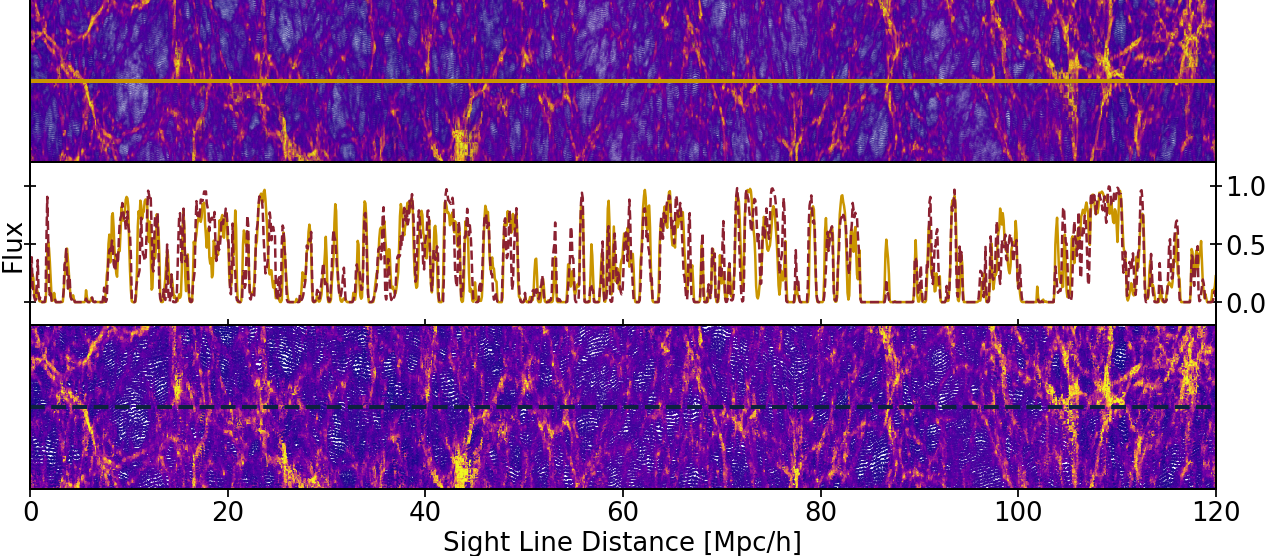
\includegraphics[width=\columnwidth]{figures/spectra_temp_simulation.png}
    \caption{\label{fig:spec_sim}
    Example Lyman-$\alpha$ forest spectra and corresponding gas density and temperature (colors in top and bottom panels) from an LF and HF simulation at redshift $z=4$.
    The top panel shows high resolution and the bottom panel shows low resolution.
    The middle panel shows the \lya forest spectra for the skewers passing through the middle of the top panel (high resolution, yellow line) and bottom panel (low resolution, red dashed line).
    }
\end{figure}

The range given for the gas mass resolution is due to the varying value of $h$ in our simulation suite ($\Omega_b h^2$ is fixed at a value of $0.0224$).
We show in Ref.~\cite{2023simsuite} that this gas mass is sufficient for the scales and redshifts probed by the eBOSS flux power spectrum.
Our simulations include a full galaxy physics model with star formation, stellar and AGN feedback and inhomogeneous reionization models.
Simulations were performed using MP-Gadget\footnotemark, an N-body and smoothed particle hydrodynamics (SPH) code.\footnotetext{\url{https://github.com/MP-Gadget/MP-Gadget}}
MP-Gadget uses the gravitational timestepping algorithm from Gadget-4 \cite{Springel:2021}, and various other algorithmic improvements \cite{2020JCAP...06..002B}.
Simulations are initialised at $z=99$ and finish at $z=2.2$. The galaxy formation model is similar to the \texttt{ASTRID} simulation \cite{2022MNRAS.512.3703B, 2022MNRAS.513..670N} and is described fully in Ref.~\cite{2023simsuite}.


\subsection{Cosmological \& Astrophysical Parameters}\label{sec:parameters}

Table~\ref{tab:emulatorparams} summarises the parameters that are varied across our suite of simulations, as well as their limits.
We model the primeval (that is, the pre-transfer function) power spectrum $P(k)$  using two parameters: a slope, $n_P$, and an amplitude, $A_P$:
\begin{equation}
    P(k) = A_P \left(\frac{k}{0.78\, \mathrm{Mpc}^{-1}}\right)^{n_P - 1}\,.
\end{equation}
The simulation initial conditions are then generated using a set of transfer functions from CLASS. This parameterization is the same as that used by Planck, but with a different pivot scale, $0.78\, \mathrm{Mpc}^{-1}$, rather than $0.05 \,\mathrm{Mpc}^{-1}$, reflecting the smaller scales probed by the forest.

We also vary the Hubble parameter $h$, and the total matter density through $\Omega_M h^2$, although we will see these are not strongly constrained by the \Lya~forest.
We add three parameters for the He~{\sc ii} reionization model \cite{2020MNRAS.496.4372U}: $z_{Hei}$ and $z_{Hef}$ are the redshifts for the start and end of He~{\sc ii} reionization, and $\alpha_q$ is the quasar spectral index (which scales the peak temperature during He~{\sc ii} reionization).
$z_{Hi}$ is the midpoint redshift of H~{\sc i} reionization.
Finally, $\epsilon_{AGN}$ is the black hole feedback factor, to which the \lya~forest is insensitive.

\begin{table*}
\begin{centering}
  \begin{tabular}{llll}
  \hline
  Parameter & Minimum & Maximum & Description \\
    \hline
    $n_P$  &  $0.8$  & $0.995$ & Scalar spectral index \\
    $A_P$  &  $1.2 \times 10^{-9}$  & $2.6 \times 10^{-9}$ & Power amplitude at $k = 0.78 \,\mathrm{Mpc}^{-1}$ \\
    $h$    & $0.65$  & $0.75$ & Hubble parameter \\
    $\Omega_0 h^2$ & $0.14$ & $0.146$ & Total matter density \\
    $z_{Hei}$      & $3.5$  & $4.1$  & Start redshift of HeII reionization \\
    $z_{Hef}$      & $2.6$  & $3.2$  & End redshift of HeII reionization \\
    $\alpha_q$     & $1.3$  & $2.5$ & Quasar spectral index during HeII reionization  \\
    $z_{Hi}$        & $6.5$ & $8$   & Median redshift of HI reionization \\
    $\epsilon_{AGN}$ & $0.03$ & $0.07$ & Thermal efficiency of black hole feedback \\
    $\tau_0$ & $0.75$ & $1.25$ & Mean optical depth at $z=3$ in Eq.~\ref{eq:meanflux}.\\
    $d \tau_0$ & $-0.4$ & $0.25$ & Mean optical depth redshift evolution in Eq.~\ref{eq:meanflux}. \\
    \hline
  \end{tabular}
  \caption{Summary of likelihood function parameters, together with the ranges covered by the emulator. We vary a total of $11$ parameters: $4$ for cosmology, $3$ for the helium reionization model, $1$ for the hydrogen reionization model, $1$ for the strength of AGN feedback and $2$ for the mean optical depth.}
  \label{tab:emulatorparams}
  \end{centering}
\end{table*}

There are two further parameters for the \Lya~effective optical depth, varied by post-processing the artificial spectra.
We parameterize the mean flux $\mathcal{F} = \exp(-\tau)$ by modifying the power law redshift evolution from Ref.~\cite{2007MNRAS.382.1657K}, as
\begin{align}
\tau^{\text{Kim}}_{\text{H~{\sc i}}}(z) &= 0.0023 \times (\tau_{z=3})\times (1+z)^{3.65}\,, \\
\tau^{\text{eff}}_{\text{H~{\sc i}}}(z) &= \tau_0 \left(\frac{\tau^{\text{Kim}}_{\text{H~{\sc i}}}(z)}{\tau^{\text{Kim}}_{\text{H~{\sc i}}}(3)}\right)^{d\tau_0} \tau^{\text{Kim}}_{\text{H~{\sc i}}}(z)\,.
 \label{eq:meanflux}
\end{align}
The parameters varied are $\tau_0$ and $d\tau_0$, with $(1, 0)$ corresponding to the redshift evolution of Ref.~\cite{2007MNRAS.382.1657K}. $\tau_0$ is normalised at $z=3$ so that $d\tau_0 > 0$ corresponds to a higher optical depth at $z > 3$ and a lower optical depth at $z < 3$. $\tau_0$ changes the normalisation of the optical depth at $z=3$. We choose prior ranges for $\tau_0$ and $d\tau_0$ that comfortably cover the measurement error: $0.75 < \tau_0 < 1.25$ and $-0.4 < d\tau_0 < 0.25$.
As the mean flux is chosen in post-processing, we can dramatically over-sample these parameters. We sample $10$ linearly spaced values of the mean flux. Sampling values are independent of redshift and are chosen to cover the range of $\tau_0$ and $d\tau_0$ at the extreme ($z=2.2$ and $z=4.6$) redshifts included in eBOSS.
The final set of flux power spectra is thus ten times the number of simulations, or $480$ LF, and $30$ HF simulated flux power spectra.
We have freedom to vary the \Lya~mean flux as it is degenerate with the amplitude of the ultraviolet background (UVB). 

% --------------------------------------------------------------------------------------------------

\subsection{Summary Statistics: Flux Power and IGM Temperature}\label{sec:sim_fps}

Figure~\ref{fig:spec_sim} shows an example of the gas density and temperature (colors) at $z=4$ for both high and low resolution in our simulations, demonstrating how spectra connect to the matter density field.
We generate a total of $3\times 480^2 = 691,200$ spectra from each snapshot of each simulation, from $z=4.6$ to $z=2.2$ in increments of $\Delta z=0.2$, with a pixel resolution of $10$ km s$^{-1}$.
We generate \lya forest absorption spectra using Fake Spectra Flux Extractor \cite{2017ascl.soft10012B}\footnotemark, described in Ref.~\cite{2015MNRAS.447.1834B}.
\footnotetext{\url{https://github.com/sbird/fake_spectra}}
We compute the 1D flux power spectrum of the \Lya~forest flux, averaged over all sightlines.
The flux power is defined as 
\begin{equation}
 P_F(k) = |L^{-1}\tilde{\delta}^2_F(k)|\,.   
\end{equation}
$\tilde{\delta}^2_F(k)$ is the Fourier transform of the flux excess, $\delta_F(k) = F(k)/\langle F(k) \rangle - 1$, and $L$ is the length of the sightline. 

Our simulations contain a realistic population of DLAs, which we mask as in the observational pipeline.
We extract the IGM temperatures at mean density directly from the simulation snapshots.
First, the temperature and density for all the gas particles in the simulation are retrieved, then all particles that are within $5\%$ of the critical density are retained.
The median temperature of these retained particles is the IGM temperature at mean density.
All of the \lya forest flux power spectra, IGM temperatures, trained emulators, as well as select MCMC chains are available \footnote{\url{https://github.com/mafern/InferenceLyaData}}.

%--------------------------------------------------------------------------------------------------
% --------------------------------------------------------------------------------------------------
% --------------------------------------------------------------------------------------------------
% --------------------------------------------------------------------------------------------------
% --------------------------------------------------------------------------------------------------

\subsection{Gaussian Process Emulators}\label{sec:gps}

We use the Gaussian Process (GP) emulators described in Refs.~\cite{2022MNRAS.517.3200F, 2023simsuite} for the 1D flux power spectra and mean IGM temperature extracted from our simulations.
The emulators interpolate over simulation outputs and make predictions for arbitrary parameter sets within the parameter limits shown in Table~\ref{tab:emulatorparams}.
We use a multi-fidelity model, which allows simulations with different particle loads, and thus costs, to be combined together.
Specifically, we combine simulations run at two different resolutions, high fidelity (HF) and low fidelity (LF) specified in Table~\ref{table:simulations}. 
The multi-fidelity prediction for the HF outputs (shown here for the \lya forest flux power spectrum, but equally valid for the IGM temperature) is given by a linear multi-fidelity model, at each redshift:
\begin{equation}
    P_F^{^\mathrm{HF}}(k, \boldsymbol{\theta} | z) = \rho_z \cdot P_F^{^\mathrm{LF}}(k, \boldsymbol{\theta} | z) + \delta(k, \boldsymbol{\theta} | z),
    \label{eq:ko_model}
\end{equation}
where $\rho_z$ is a constant parameter, and $\delta(k, \boldsymbol{\theta} | z)$ is a GP.
We have simplified the model from Ref.~\cite{2022MNRAS.517.3200F} by dropping the $k$ dependence in $\rho_z$.
All cosmology and scale dependence is thus in the additive GP $\delta(k, \boldsymbol{\theta} | z)$.
\maf{We tested a GP emulator that included scale dependence in the $\rho$ term, but found that this did not significantly improve the accuracy of the predictions.}
We train the GP emulators separately for each redshift. We implement our multi-fidelity models using Emukit \cite{2021arXiv211013293P}.

Ref.~\cite{2023simsuite} quantifies the accuracy of our emulator using a leave-one-out technique, in which one simulation is chosen as a `left out' sample.
A smaller emulator built excluding all samples from this simulation is used to predict the summary statistic for the left out sample.
After computing leave-one-out interpolation errors for all potential test samples, we found on average $0.2\%$ accuracy for the low-fidelity simulations and $1\%$ for the high fidelity simulations.
The last is likely a significant over-estimate of the actual error since the leave-one-out procedure in this case is missing $1/3$ of the total training data.
The emulator accuracy indicates that the emulators are performing well, with potential errors significantly smaller than the $7\%$ average uncertainty in mean IGM temperature measurements \cite{2019JCAP...07..017C}.
Our likelihood function and emulator code is publicly available\footnote{\url{https://github.com/sbird/lya_emulator_full}}.

% --------------------------------------------------------------------------------------------------